\documentclass[11pt]{article}
\usepackage[margin=1in]{geometry}
\usepackage[T1]{fontenc}
\usepackage{lmodern}
\usepackage{amsmath,amssymb,booktabs,graphicx}
\usepackage[round]{natbib}
\usepackage[hidelinks]{hyperref}

% Result numbers and process facts. Generated by `crew.py numbers`; never typed by hand.
% Generated by `crew.py numbers` from claims.jsonl. Do not edit by hand.
% Each macro is a number taken from a logged run; see claims.jsonl.
\newcommand{\IvReturn}{0.1324}  % iv-return
\newcommand{\IvReturnSe}{0.0493}  % iv-return-se
\newcommand{\IvReturnSeRobust}{0.0488}  % iv-return-se-robust
\newcommand{\IvReturnPct}{14.2}  % iv-return-pct
\newcommand{\FirstStage}{0.3639}  % first-stage
\newcommand{\FirstStageSe}{0.1024}  % first-stage-se
\newcommand{\ReducedForm}{0.0346}  % reduced-form
\newcommand{\ReducedFormSe}{0.0173}  % reduced-form-se
\newcommand{\OlsReturn}{0.0726}  % ols-return
\newcommand{\OlsReturnSe}{0.0037}  % ols-return-se
\newcommand{\NSample}{3,010}  % n-sample
\newcommand{\BFiveIv}{0.1224}  % b5-iv
\newcommand{\BFiveIvSe}{0.0465}  % b5-iv-se
\newcommand{\BOneFs}{0.3924}  % b1-fs
\newcommand{\BOneFsSe}{0.1138}  % b1-fs-se
\newcommand{\BThreeRf}{0.0325}  % b3-rf
\newcommand{\BThreeRfSe}{0.0174}  % b3-rf-se
\newcommand{\ASixIv}{0.1404}  % a6-iv
\newcommand{\ASixIvSe}{0.0552}  % a6-iv-se
\newcommand{\ASixIvSeRobust}{0.0546}  % a6-iv-se-robust
\newcommand{\ASixFs}{0.3224}  % a6-fs
\newcommand{\ASixFsSe}{0.0834}  % a6-fs-se
\newcommand{\ASixRf}{0.0453}  % a6-rf
\newcommand{\ASixRfSe}{0.0179}  % a6-rf-se
\newcommand{\AFiveIv}{0.1315}  % a5-iv
\newcommand{\AFiveIvSe}{0.0550}  % a5-iv-se
\newcommand{\AFiveIvSeRobust}{0.0541}  % a5-iv-se-robust
\newcommand{\AFiveFs}{0.3199}  % a5-fs
\newcommand{\AFiveFsSe}{0.0879}  % a5-fs-se
\newcommand{\AFiveRf}{0.0421}  % a5-rf
\newcommand{\AFiveRfSe}{0.0181}  % a5-rf-se
\newcommand{\AFiveOls}{0.0747}  % a5-ols
\newcommand{\AFiveOlsSe}{0.0035}  % a5-ols-se
\newcommand{\AFiveArHomLo}{0.0248}  % a5-ar-hom-lo
\newcommand{\AFiveArHomHi}{0.2848}  % a5-ar-hom-hi
\newcommand{\ASixFConv}{14.94}  % a6-f-conv
\newcommand{\ASixFEff}{15.95}  % a6-f-eff
\newcommand{\ASixArLo}{0.0395}  % a6-ar-lo
\newcommand{\ASixArHi}{0.2902}  % a6-ar-hi
\newcommand{\ASixRfTRobust}{2.62}  % a6-rf-t-robust
\newcommand{\AFiveFConv}{13.26}  % a5-f-conv
\newcommand{\AFiveFEff}{14.14}  % a5-f-eff
\newcommand{\AFiveArLo}{0.0282}  % a5-ar-lo
\newcommand{\AFiveArHi}{0.2812}  % a5-ar-hi
\newcommand{\AFiveRfTRobust}{2.40}  % a5-rf-t-robust
\newcommand{\BSixArRobLo}{-0.0068}  % b6-ar-rob-lo
\newcommand{\BSixArRobHi}{0.4983}  % b6-ar-rob-hi
\newcommand{\BSixArRobNpieces}{1}  % b6-ar-rob-npieces
\newcommand{\BSixArGkmcLo}{0.0401}  % b6-ar-gkmc-lo
\newcommand{\BSixArGkmcHi}{0.2811}  % b6-ar-gkmc-hi
\newcommand{\BSixArGkmOneNineLo}{0.0401}  % b6-ar-gkm19-lo
\newcommand{\BSixArGkmOneNineHi}{0.2811}  % b6-ar-gkm19-hi
\newcommand{\BSixArGkmOneNineqLo}{0.0401}  % b6-ar-gkm19q-lo
\newcommand{\BSixArGkmOneNineqHi}{0.2811}  % b6-ar-gkm19q-hi
\newcommand{\BSixKappaOne}{6,048}  % b6-kappa1
\newcommand{\BSixKappaOneMin}{5,320}  % b6-kappa1-min
\newcommand{\BSixRobMAtZero}{7.30}  % b6-rob-m-at-zero
\newcommand{\ASixPacoefChrBreakdown}{0.0114}  % a6-pacoef-chr-breakdown
\newcommand{\ASixPacoefChrShare}{0.253}  % a6-pacoef-chr-share
\newcommand{\ASixPacoefChrWaldBreakdown}{0.0124}  % a6-pacoef-chr-wald-breakdown
\newcommand{\AFivePacoefChrBreakdown}{0.0077}  % a5-pacoef-chr-breakdown
\newcommand{\AFivePacoefChrShare}{0.184}  % a5-pacoef-chr-share
\newcommand{\AFivePacoefChrWaldBreakdown}{0.0093}  % a5-pacoef-chr-wald-breakdown
\newcommand{\ASixPacoefCfT}{-1.32}  % a6-pacoef-cf-t
\newcommand{\ASixPacoefCfP}{0.186}  % a6-pacoef-cf-p
\newcommand{\ASixPacoefDiff}{0.0678}  % a6-pacoef-diff
\newcommand{\ASixPacoefDiffSe}{0.0547}  % a6-pacoef-diff-se
\newcommand{\ASixPacoefDiffLo}{-0.0394}  % a6-pacoef-diff-lo
\newcommand{\ASixPacoefDiffHi}{0.1749}  % a6-pacoef-diff-hi
\newcommand{\ASixOlsInPacoefAr}{1}  % a6-ols-in-pacoef-ar
\newcommand{\ASixPacoefHausmanTConv}{1.23}  % a6-pacoef-hausman-t-conv
\newcommand{\AFivePacoefCfT}{-1.10}  % a5-pacoef-cf-t
\newcommand{\AFivePacoefCfP}{0.271}  % a5-pacoef-cf-p
\newcommand{\AFivePacoefDiff}{0.0568}  % a5-pacoef-diff
\newcommand{\AFivePacoefDiffSe}{0.0542}  % a5-pacoef-diff-se
\newcommand{\AFivePacoefDiffLo}{-0.0494}  % a5-pacoef-diff-lo
\newcommand{\AFivePacoefDiffHi}{0.1630}  % a5-pacoef-diff-hi
\newcommand{\AFiveOlsInPacoefAr}{1}  % a5-ols-in-pacoef-ar
\newcommand{\AFivePacoefHausmanTConv}{1.04}  % a5-pacoef-hausman-t-conv
\newcommand{\HOnePrimaryReproduced}{5}  % h1-primary-reproduced
\newcommand{\HOneSecondaryReproduced}{19}  % h1-secondary-reproduced
\newcommand{\HTwoASixSyAbove}{0}  % h2-a6-sy-above
\newcommand{\HTwoASixMopAbove}{0}  % h2-a6-mop-above
\newcommand{\HThreeaASixPacoefPositive}{1}  % h3a-a6-pacoef-positive
\newcommand{\HFiveASixPacoefEqualityRejected}{0}  % h5-a6-pacoef-equality-rejected
\newcommand{\HTwoAFiveSyAbove}{0}  % h2-a5-sy-above
\newcommand{\HTwoAFiveMopAbove}{0}  % h2-a5-mop-above
\newcommand{\HThreeaAFivePacoefPositive}{1}  % h3a-a5-pacoef-positive
\newcommand{\HFiveAFivePacoefEqualityRejected}{0}  % h5-a5-pacoef-equality-rejected
\newcommand{\HThreebBSixReturnPositive}{0}  % h3b-b6-return-positive
\newcommand{\YoungIv}{0.0944}  % young-iv
\newcommand{\YoungIvSe}{0.0645}  % young-iv-se
\newcommand{\YoungOls}{0.0745}  % young-ols
\newcommand{\YoungOlsSe}{0.0061}  % young-ols-se
\newcommand{\YoungN}{2,037}  % young-n
\newcommand{\BalKwwYoung}{0.244}  % bal-kww-young
\newcommand{\BalKwwYoungSe}{0.651}  % bal-kww-young-se
\newcommand{\BalKwwYoungSdu}{0.032}  % bal-kww-young-sdu
\newcommand{\BalKwwYoungN}{753}  % bal-kww-young-n
\newcommand{\BalKwwAll}{0.685}  % bal-kww-all
\newcommand{\BalKwwAllSe}{0.305}  % bal-kww-all-se
\newcommand{\BalKwwAllSdu}{0.080}  % bal-kww-all-sdu
\newcommand{\BalIq}{0.605}  % bal-iq
\newcommand{\BalIqSe}{0.709}  % bal-iq-se
\newcommand{\BalIqSdu}{0.039}  % bal-iq-sdu
\newcommand{\BalIqN}{2,061}  % bal-iq-n
\newcommand{\IqObsDiff}{0.083}  % iq-obs-diff
\newcommand{\IqObsDiffSe}{0.019}  % iq-obs-diff-se
\newcommand{\ASixRfSeCl}{0.0142}  % a6-rf-se-cl
\newcommand{\ASixRfTCl}{3.18}  % a6-rf-t-cl
\newcommand{\AFiveRfSeCl}{0.0151}  % a5-rf-se-cl
\newcommand{\AFiveRfTCl}{2.78}  % a5-rf-t-cl
\newcommand{\NClusters}{18}  % n-clusters
\newcommand{\MinClusterSize}{25}  % min-cluster-size
\newcommand{\TCritCl}{2.110}  % t-crit-cl

% Generated by `crew.py numbers` from reviews/, runs/ and replication.json. Do not edit by hand.
% Use these macros for any statement about how the paper was made (rounds, runs, rerun).
\newcommand{\CrewReviewRounds}{13}  % review records in reviews/
\newcommand{\CrewRoundsQuestion}{2}  % rounds of the question review
\newcommand{\CrewRoundsLiterature}{2}  % rounds of the literature review
\newcommand{\CrewRoundsDesign}{3}  % rounds of the design review
\newcommand{\CrewRoundsCode}{4}  % rounds of the code review
\newcommand{\CrewRoundsResults}{2}  % rounds of the results review
\newcommand{\CrewRoundsPaper}{0}  % rounds of the paper review
\newcommand{\CrewFindingsCritical}{0}  % critical findings raised, summed over rounds
\newcommand{\CrewFindingsMajor}{22}  % major findings raised, summed over rounds
\newcommand{\CrewFindingsMinor}{76}  % minor findings raised, summed over rounds
\newcommand{\CrewReviewerModels}{claude-opus-5-5}  % models the Reviewer ran on
\newcommand{\CrewReviewIndependence}{fresh-context}  % how independent the reviews were
\newcommand{\CrewRuns}{18}  % runs in the ledger
\newcommand{\CrewRunsAnalysis}{15}  % analysis runs
\newcommand{\CrewRunsDataPrep}{3}  % data-prep runs
\newcommand{\CrewRunsSuperseded}{3}  % runs replaced by a later run with the same id (archived)
\newcommand{\CrewRunsUnreviewed}{0}  % analysis runs not covered by a passing code review
\newcommand{\CrewResultClaims}{159}  % result claims
\newcommand{\CrewCitationClaims}{46}  % citation claims
\newcommand{\CrewRerunReproduced}{0}  % runs the clean rerun reproduced
\newcommand{\CrewRerunTotal}{0}  % runs the clean rerun re-executed
\newcommand{\CrewRerunStatus}{not run}  % outcome of the latest clean rerun


\setlength{\emergencystretch}{3em}
\renewcommand{\topfraction}{0.9}
\renewcommand{\textfraction}{0.07}
\renewcommand{\floatpagefraction}{0.8}
\newcommand{\var}[1]{\texttt{#1}}
% Number of H1 misses, derived from the count macros (no run metric holds it).
\newcommand{\HOneMisses}{\the\numexpr\HOnePrimaryTargets+\HOneSecondaryTargets-\HOnePrimaryReproduced-\HOneSecondaryReproduced\relax}

\title{Does Card's College-Proximity Estimate of the Return to Schooling\\
Replicate and Survive Weak-Instrument-Robust Inference?\\[4pt]
\large A Replication of Card (1993), NBER Working Paper 4483}
\author{Bryce Wang (human PI) \\ \small Drafted with Free-Research-Crew; see the AI-use statement.}
\date{\today}

\begin{document}
\maketitle

\begin{abstract}
\noindent
We replicate the OLS and instrumental-variables estimates of the return to schooling in
Card's college-proximity paper (NBER Working Paper 4483, 1993; published 1995) from his
public extract of the NLS Young Men, with targets, standard-error formulas and decision
rules fixed before any estimate was computed. In Card's basic specification the 2SLS
coefficient on schooling is \IvReturn{} (standard error \IvReturnSe{}) on \NSample{} men,
reproducing the published 0.132 (0.049); the OLS coefficient \OlsReturn{} reproduces 0.073. % crew:literal
Of the \HOnePrimaryTargets{} primary and \HOneSecondaryTargets{} secondary printed targets,
\HOnePrimaryReproduced{} and \HOneSecondaryReproduced{} are reproduced. All \HOneMisses{}
misses lie in the first-stage and reduced-form columns of Card's Panel~B; a post hoc
regression that keeps experience as an endogenous regressor instrumented by age matches
\DiagTargetsReproduced{} of the \DiagTargets{} printed numbers there, which is consistent
with, but does not prove, how they were estimated. A heteroskedasticity-robust
Anderson--Rubin projection set, valid whatever the instrument strength but conservative,
runs from \BSixArRobLo{} to \BSixArRobHi{} for the return in the basic specification: it
contains zero, so a positive return is not established by this test. Homoskedastic
subvector sets exclude zero but were fixed in advance not to decide; their statistic at a
zero return is not larger than the robust one, so the two decisions differ through the
critical values (the projection's is the more conservative), not through
heteroskedasticity. In the specifications that treat experience as exogenous, the
first stage is below the usual weak-instrument thresholds, the robust Anderson--Rubin set
for the Panel~A coefficient on schooling lies above zero, it first includes zero once
proximity may raise log wages directly by \ASixPacoefChrBreakdown{} (about one log point),
and equality of the 2SLS and OLS coefficients is not rejected. The 2SLS coefficient is not
the average return to schooling for all men.
\end{abstract}

\section{Introduction}
\label{sec:intro}

\citet{card1993nber} used the presence of a four-year college in a young man's local labor
market in 1966 as an instrument for his completed schooling. In his basic specification,
on 3,010 men from the 1976 wave of the National Longitudinal Survey of Young Men, the % crew:literal
instrumental-variables (IV) estimate of the log-wage return to a year of schooling is 0.132 % crew:literal
(standard error 0.049), against an OLS estimate of 0.073 (0.004) % crew:literal
\citep[Table~3 Panel~B column~6; Table~2 column~5]{card1993nber}. Card noted that the IV
estimates are imprecise and that one cannot reject that the gap between IV and OLS is
sampling error \citep[p.~13]{card1993nber}. The paper circulated as NBER Working Paper 4483
and was published in 1995 as a book chapter \citep{card2000estimating}; Card's own codebook
and the seed task cite it as Working Paper 4832, which is a different paper
\citep{card1994earnings}. We could not read the chapter, so every published number below
is from the working paper. Card's later survey quotes the same headline estimates for the
chapter \citep{card2000estimating}.

This paper asks two questions. The first is computational: does a logged replication, built to be rerun from scratch, from Card's public file \citep{cardproximitydata} reproduce the published OLS,
first-stage, reduced-form and 2SLS estimates? \citet{kling2001interpreting} reported an
exact replication of the basic specification (OLS 0.073, IV 0.132 (0.049)), and several % crew:literal
later papers reproduce the specifications that treat experience as exogenous
\citep{bi2020inferring,blandhol2025tsls,delbianco2026testing}. A successful reproduction is
therefore a check, not new evidence on the return to schooling. The second question is
how much of the IV conclusion survives inference that is robust to a weak instrument (for
Card's basic specification and for the specifications that treat experience as exogenous)
and, for the latter only, to a bounded violation of the exclusion restriction.

The answers are as follows. The 2SLS estimate of Card's basic specification is reproduced
to the printed digit: \IvReturn{} (\IvReturnSe{}), with OLS \OlsReturn{}
(\OlsReturnSe{}) and N $=$ \NSample{}. Of the \HOnePrimaryTargets{} primary targets fixed
in advance, \HOnePrimaryReproduced{} are reproduced; of \HOneSecondaryTargets{} secondary
targets, \HOneSecondaryReproduced{}. Every miss is a first-stage or reduced-form coefficient (or its
standard error) in Card's Panel~B, where experience is treated as endogenous; all
Panel~A numbers, both OLS columns and both Panel~B 2SLS estimates are reproduced. A post
hoc diagnostic, labelled as such throughout, finds that Card's printed Panel~B columns 1--4
match regressions that keep experience in the equation as an endogenous regressor
instrumented by age (Section~\ref{sec:diag}).

On inference, the result that bears on the return to schooling in Card's basic
specification is negative in the narrow sense fixed before the runs: the
heteroskedasticity-robust projection Anderson--Rubin set, [\BSixArRobLo,
\BSixArRobHi], contains zero, so this test does not establish that the return is
positive. It is not evidence that the return is zero. The homoskedastic subvector
statistic at a zero return, \BSixHomStatAtZero{}, is not larger than the robust projection
statistic there, \BSixRobMAtZero{}, so the robust and homoskedastic sets disagree about zero
through their critical values (the projection's $\chi^2_3$ value is the more conservative),
not because heteroskedasticity-robust inference is less favourable to a positive return
(a post hoc, descriptive comparison that changes neither the decision rule nor the primary
set). The homoskedastic subvector sets of
\citet{guggenberger2012asymptotic} and \citet{guggenberger2019more} exclude zero, but they
assume homoskedasticity and were fixed in advance not to decide. Everything that comes out
positive concerns the Panel~A coefficient, which assumes experience exogenous although
experience is age minus schooling minus six: the robust Anderson--Rubin set for that
coefficient with family background is [\ASixArLo, \ASixArHi], its first stage is below the
Stock--Yogo and Montiel Olea--Pflueger thresholds, the set first includes zero if
proximity may raise log wages directly by \ASixPacoefChrBreakdown{} (about one log
point), and the 2SLS and OLS coefficients are not distinguishable.

The contribution is small and stated precisely. Weak-instrument-robust inference and
exclusion sensitivity on these data are published for the Panel~A specification without
family background, under homoskedasticity \citep{cinelli2025omitted}, and with a
direct-effect parameterisation for a different control set
\citep{steiner2025possibilistic}. We add the heteroskedasticity-robust effective $F$,
Anderson--Rubin set and Conley--Hansen--Rossi breakdown point on the Panel~A specification
that keeps Card's family-background controls; in the Scout's limited search these were not
reported on that column. We state that with one instrument the last two are restatements
of the reduced form. We report subvector sets for Card's basic specification, the
diagnosis of the Panel~B misses, and the correction of the working-paper number. We add no
new estimate of the return to schooling.

\section{Data}
\label{sec:data}

The data are Card's public extract \var{nls.dat} \citep{cardproximitydata}: a 1976
cross-section of the National Longitudinal Survey of Young Men, a panel that began in 1966
with men aged 14--24. The file has 3,613 men interviewed in 1976 with valid education, of % crew:literal
whom 3,010 report a valid 1976 wage \citep[pp.~3--7 and Table~1]{card1993nber}. Card's % crew:literal
wage sample keeps hourly wages between \$1 and \$30 and excludes 49 men with a missing % crew:literal
1966 interview month \citep[Table~1 note]{kling2001interpreting}. The file's log wage
\var{lwage76} is already trimmed, so our sample rule is ``non-missing \var{lwage76}'', which
gives N $=$ \NSample{}, Card's N. The regressions are unweighted, as in Card's example
program. The derived data set distributed with Wooldridge's textbook
\citep{wooldridgecarddata} lacks the parental-education classes and imputation flags, so it
cannot build Card's family-background controls; we use \var{nls.dat}.

\paragraph{Variables.} The outcome is the log hourly wage in 1976. Schooling is completed
years of education in 1976 (\var{ed76}). The instrument is an indicator for an accredited
four-year college in the local labor market in 1966, defined from county of residence
\citep[p.~5 and fn.~7]{card1993nber}. Potential experience is age minus schooling minus six,
entered as a quadratic \citep[p.~7]{card1993nber}. The base controls are a Black indicator,
indicators for southern and SMSA residence in 1976, eight indicators for region in 1966, an
SMSA-in-1966 indicator, and experience and its square; the family-background set adds 14
variables: mother's and father's years of schooling, indicators for imputed parental
schooling, eight parental-education class indicators and two family-structure indicators
at age 14 \citep[Tables~2--4 notes]{card1993nber}. Parental schooling is the file's
mean-imputed version. The KWW score (Knowledge of the World of Work, from the 1966
interview) and a school-record IQ score are used only in a balance check.

\paragraph{Summary statistics.} Table~\ref{tab:sumstats} sets Card's Table~1 description
of the wage sample next to our analysis sample. \TOneRoundsOk{} of the \TOneItems{} items
round to Card's printed values. Of the \TOneMisses{} that do not, two (the shares aged
18--20 in 1966 and living in the South in 1976) are each one man from Card's rounding: one
man fewer in the category would reproduce his figure. The third, the share of Black men,
is further from Card's figure and its cause is unknown. Card's column for the wage sample
repeats the figure of his full-sample column exactly, which suggests a transcription error
in his table, but that is a conjecture. The sample itself is not in doubt: N equals Card's,
and Card's reported mean log hourly wage of 6.262 (s.d. 0.444) and mean schooling of % crew:literal
13.263 years (s.d. 2.677) for the wage sample \citep[Tables~2--3 notes]{card1993nber} % crew:literal
agree with the analysis file. These statistics come from the analysis run
\var{describe-sample}, which recomputes the values the Data RA's preparation run recorded
before any analysis; it was added at the paper stage, after the results gate (deviation
D7), so no results review has covered it. They are univariate and relate the instrument to
neither schooling nor wages.

% Summary statistics: Card WP 4483 Table 1 column 3 against the replicated sample (run
% describe-sample, deviation D7). Published values on crew:literal lines; replicated values are macros.
\begin{table}[tbp]
\centering
\small
\caption{Summary statistics of the wage sample: Card's Table~1, column~3, and the
replicated analysis sample (N $=$ \NSample{} men with a 1976 wage). Percent of the sample
unless stated. ``Match'': the replicated value rounds to Card's at his printed precision.}
\label{tab:sumstats}
\begin{tabular}{@{}llll@{}}
\toprule
Item & Card (WP 4483) & Replicated & Match \\
\midrule
\multicolumn{4}{@{}l}{\emph{Age in 1966}} \\
\quad 14--15 & 25.5 & \TOneAgeFourteen{} & yes \\ % crew:literal
\quad 16--17 & 24.1 & \TOneAgeSixteen{} & yes \\ % crew:literal
\quad 18--20 & 24.6 & \TOneAgeEighteen{} & no$^{a}$ \\ % crew:literal
\quad 21--24 & 25.8 & \TOneAgeTwentyOne{} & yes \\ % crew:literal
\multicolumn{4}{@{}l}{\emph{Region of residence in 1966}} \\
\quad Northeast & 20.7 & \TOneNortheast{} & yes \\ % crew:literal
\quad Midwest & 26.0 & \TOneMidwest{} & yes \\ % crew:literal
\quad South & 41.4 & \TOneSouthSixtySix{} & yes \\ % crew:literal
\quad West & 11.9 & \TOneWest{} & yes \\ % crew:literal
Lived in an SMSA in 1966 & 65.0 & \TOneSmsaSixtySix{} & yes \\ % crew:literal
Grew up near a four-year college & 68.2 & \TOneNearFour{} & yes \\ % crew:literal
Lived with mother and father at 14 & 78.9 & \TOneMomDad{} & yes \\ % crew:literal
Lived with single mother at 14 & 10.1 & \TOneSingleMom{} & yes \\ % crew:literal
Mother's education, years (not imputed) & 10.3 & \TOneMomEd{} & yes \\ % crew:literal
Father's education, years (not imputed) & 10.0 & \TOneDadEd{} & yes \\ % crew:literal
Black & 23.0 & \TOneBlack{} & no$^{b}$ \\ % crew:literal
KWW score, men with a score & 33.5 & \TOneKww{} & yes \\ % crew:literal
Years of education in 1976 & 13.3 & \TOneEdSeventySix{} & yes \\ % crew:literal
Lived in the South in 1976 & 40.3 & \TOneSouthSeventySix{} & no$^{a}$ \\ % crew:literal
\midrule
\multicolumn{4}{@{}l}{Items that round to Card's value: \TOneRoundsOk{} of \TOneItems{}; not matched: \TOneMisses{}.} \\
\bottomrule
\end{tabular}

\smallskip
\begin{minipage}{0.95\linewidth}
\footnotesize
\emph{Notes.} Recomputed by the run \var{describe-sample} (deviation D7, added at the paper
stage), which asserts equality with the values the data-preparation run recorded. Regions
1966 group the nine unnamed codebook regions as Northeast 1--2, Midwest 3--4, South 5--7,
West 8--9, an inference of the Data RA. Parental education is averaged over men whose value
is not imputed. $^{a}$One man from the published rounding: one man fewer in the category
would round to Card's figure. $^{b}$Cause unknown. Card's column~3 repeats his
column~2 figure exactly, which suggests a transcription error in his table, but this is a
conjecture, not established.
\end{minipage}
\end{table}


\section{Empirical strategy}
\label{sec:strategy}

\paragraph{Estimating equations.} For man $i$ let $y_i$ be the log wage, $S_i$ schooling,
$X_i$ potential experience, $Z_i$ the proximity indicator, $A_i$ age in 1976 and $W_i$ the
remaining controls (with or without family background). Card's basic specification,
Panel~B, is
\begin{equation}
y_i = \beta S_i + \gamma_1 X_i + \gamma_2 X_i^2 + W_i'\delta + u_i, \label{eq:panelb}
\end{equation}
estimated by 2SLS with $S_i$, $X_i$ and $X_i^2$ endogenous and $Z_i$, $A_i$ and $A_i^2$ as
excluded instruments; column~6 includes family background and is the primary target of
this replication. The Panel~A specifications treat $X_i$ and $X_i^2$ as exogenous controls,
so that $S_i$ is the only endogenous regressor and $Z_i$ the only instrument:
\begin{equation}
S_i = \pi Z_i + V_i'\phi + v_i, \qquad
y_i = \lambda Z_i + V_i'\psi + e_i, \qquad
\beta^{A} = \lambda / \pi, \label{eq:panela}
\end{equation}
with $V_i = (X_i, X_i^2, W_i)$. We call $\beta^{A}$ the Panel~A coefficient on schooling;
it equals $\beta$ only if experience is uncorrelated with the wage error, which cannot hold
exactly when schooling is endogenous, because $X_i = A_i - S_i - 6$
\citep[p.~13]{card1993nber}. Panel~A column~6 includes family background, column~5 does
not. Neither is Card's basic specification. The OLS counterparts are Card's Table~2
column~5 (for B6 and A6) and column~2 (for A5).

\paragraph{Estimand.} $\beta$ is the coefficient on schooling in the linear model
\eqref{eq:panelb}. It is not the average return to schooling for all men. With
heterogeneous returns, IV independence assumptions identify a weighted average of per-unit
effects along the causal response function \citep{angrist1995twostage}; with proximity
independent of the unobservables conditional on the covariates and with monotonicity, the
2SLS coefficient is a weighted average of the returns of men whose schooling responds to
proximity, conditional on the covariates \citep{kling2001interpreting}. On these data both
conditions are in doubt. With additive covariates, 2SLS has that weakly causal reading
only under a ``rich covariates'' condition, which \citet{blandhol2025tsls} reject for
Panel~A column~5. For a different estimand (a binary ``some college'' treatment, without
family background, on 2,988 men) \citet{tubbicke2023when} finds 2SLS 50--100\% above
estimators that do not rely on that condition and, reporting S{\l}oczy{\'n}ski, that
allowing for defiers roughly halves 2SLS. Because experience is also instrumented in
\eqref{eq:panelb}, these complier results do not directly define whose return $\beta$
weights. We therefore read $\beta$ as the coefficient of Card's model, not as a population
average.

\paragraph{Identifying assumption.} In plain words: (i) among men with the same race,
region, urban residence and (in columns 2, 4, 6) family background, growing up near a
four-year college is unrelated to the unobserved determinants of 1976 wages and affects
wages only through schooling, and it does shift schooling; (ii) in Panel~B, age affects
wages only through experience, given the controls (no separate age or cohort effect),
whereas Panel~A instead assumes experience itself is exogenous. What would violate (i):
families who value schooling choosing to live near colleges, better local schools near
colleges, local wage premia not absorbed by the region and SMSA controls, and older men
having moved near a college by 1966 for college itself; Card names all four
\citep[pp.~16--18]{card1993nber}. In the data, (i) would be contradicted by proximity
predicting the 1966 KWW score of men aged 14--15 (before college) or the school-record IQ
score given the controls, by an estimate that depends on men old enough in 1966 to have
moved for college, and by large movement when family background is added. The age
exclusion in (ii) is maintained, as in Card, and nothing here tests it. None of these
checks can confirm the assumptions.

\paragraph{Replication targets (H1).} Card does not state his standard-error formula. We
fixed conventional (homoskedastic, $n-k$) standard errors for the comparison, because
\citet{blandhol2025tsls} obtain 0.054 for Panel~A column~5 with robust errors where Card % crew:literal
prints 0.055, and report HC1 standard errors alongside. A printed number counts as % crew:literal
reproduced if the unrounded replicated value rounds to it at the printed precision; N must
match exactly. The \HOnePrimaryTargets{} primary targets are the B6 2SLS estimate, the B2 first stage, the B4
reduced form and the Table~2 column~5 OLS estimate, each with its standard error, and N;
the \HOneSecondaryTargets{} secondary targets are every other printed proximity or schooling coefficient of
Table~3 and Table~2 columns 2 and 5, with standard errors, and the homoskedastic
Anderson--Rubin set that \citet{cinelli2025omitted} print for Panel~A column~5.

\paragraph{Inference (H2--H5).} All of it was fixed at the design gate and uses HC1
standard errors.
\begin{itemize}
\item \emph{H2, instrument strength} (Panel~A column~6 primary, column~5 alongside): the
conventional first-stage $F$ against the Stock--Yogo 10\% maximal-size value 16.38, which
assumes homoskedasticity \citep{stock2002testing,stock2005testing}, and the effective $F$ of
\citet{montielolea2013robust}, which with one instrument equals the robust first-stage $F$,
against its 5\%-size, 10\%-worst-case-bias value 23.11. Neither threshold applies to the
three-endogenous-regressor Panel~B, for which no strength test is reported.
\item \emph{H3(a), Panel~A}: the robust Anderson--Rubin (AR) set
$\{b_0 : (\hat\lambda - b_0\hat\pi)^2 / (V_{\lambda\lambda} - 2b_0V_{\lambda\pi} +
b_0^2V_{\pi\pi}) \le 3.841\}$, valid whatever the instrument strength
\citep{anderson1949estimation,andrews2019weak}, which \citet{andrews2019weak} recommend
reporting with one instrument whatever the first-stage $F$. With one instrument the set
excludes 0 exactly when the robust reduced-form $t$ test rejects. The decision rule: the
statement ``the Panel~A coefficient on schooling is positive'' survives only if the set is
one bounded interval above 0.
\item \emph{H3(b), Card's basic specification}: a subvector AR set for $\beta$ with
$(\gamma_1,\gamma_2)$ as nuisance parameters. Primary, because it is robust to
heteroskedasticity: the projection set $\{b_0 : \min_g \mathrm{HAR}(b_0, g) \le 7.815\}$,
where $\mathrm{HAR}$ is the HC1 full-vector AR statistic and 7.815 the $\chi^2_3$ 95\%
value. Projection sets are valid but often conservative \citep{andrews2019weak}.
Alongside, not deciding: the homoskedastic subvector AR set with $\chi^2_1$ critical values
\citep[GKMC]{guggenberger2012asymptotic}, and the same statistic with the data-dependent
critical values of \citet[GKM19]{guggenberger2019more}, which depend on the largest root
$\kappa_1$ and rise towards the $\chi^2_1$ value 3.841 as $\kappa_1$ grows. Both rely on
homoskedasticity, and GKM19 state that under arbitrary heteroskedasticity both have size
above the nominal level. A robust conditional test exists \citep{guggenberger2024powerful},
but we found no implementation in Python, and \var{ivmodels}, which we use for the
homoskedastic sets, has no robust option \citep{ivmodelsapi,londschien2026weak}. The rule
``the return to schooling is positive'' survives only if the robust projection set is one
bounded interval above 0; a set that contains 0 is reported as ``not established'', not as
evidence of no return.
\item \emph{H4, exclusion}: following \citet{conley2012plausibly}, proximity may raise log
wages directly by $\gamma \in [0, \delta]$; the union over $\gamma$ of the robust AR sets
for the Panel~A coefficient gives the smallest $\delta^*$ at which the union includes 0.
With one instrument $\delta^* = \hat\lambda - 1.96\,\mathrm{se}(\hat\lambda)$, the lower
95\% limit of the robust reduced form, so the breakdown point is a restatement of the
reduced form. The Wald-based union, which is not robust to a weak instrument, is secondary.
\item \emph{H5, IV versus OLS}: a robust control-function test that the Panel~A 2SLS and OLS
coefficients are equal, with a 95\% Wald interval of the difference from the stacked
influence functions of the two estimators. The minimum detectable difference at 80\% power
from Card's published standard errors is about 0.154, against published differences of % crew:literal
0.067 (column~6) and 0.057 (column~5), so a non-rejection was expected and is read through % crew:literal
the interval. A difference is reported descriptively, not as a measure of ability bias.
\end{itemize}

\paragraph{Report-only checks.} Card's Table~4 row~7 (men aged 14--19 in 1966); balance of
proximity on KWW at ages 14--15, on KWW for all men and on IQ, with IQ missingness by
proximity; standard errors clustered on region-1966 $\times$ SMSA-1966 cells; and, only
after every claim of the approved plan was written, a comparison with the output listing of
Card's own SAS program (Section~\ref{sec:diag} gives the timing of later claims). Their readings were fixed in advance and none of them can change a claim.

\section{Results}
\label{sec:results}

\subsection{Reproduction of the published estimates (H1)}
\label{sec:h1}

% H1: published and replicated estimates. Replicated numbers are macros from numbers.tex;
% published numbers (Card 1993, WP 4483; Cinelli and Hazlett 2025) sit on crew:literal lines.
\begin{table}[tbp]
\centering
\small
\caption{Published and replicated estimates (H1). Coefficient with its conventional
($n-k$) standard error in parentheses; N $=$ \NSample{} men with a 1976 wage, unweighted.
A printed number is reproduced if the unrounded replicated value rounds to it at the
printed precision. ``Match'' gives the verdict for the coefficient and then for the
standard error.}
\label{tab:h1}
\begin{tabular}{@{}lllll@{}}
\toprule
Column (WP 4483) & Quantity & Published & Replicated & Match \\
\midrule
\multicolumn{5}{@{}l}{\emph{Primary targets: Card's basic specification}} \\
Table 3, B(6) & 2SLS, schooling & 0.132 (0.049) & \IvReturn{} (\IvReturnSe{}) & yes, yes \\ % crew:literal
Table 3, B(2) & first stage, proximity & 0.365 (0.105) & \FirstStage{} (\FirstStageSe{}) & no, no \\ % crew:literal
Table 3, B(4) & reduced form, proximity & 0.048 (0.019) & \ReducedForm{} (\ReducedFormSe{}) & no, no \\ % crew:literal
Table 2, col.~5 & OLS, schooling & 0.073 (0.004) & \OlsReturn{} (\OlsReturnSe{}) & yes, yes \\ % crew:literal
-- & sample size & 3,010 & \NSample{} & yes \\ % crew:literal
\addlinespace
\multicolumn{5}{@{}l}{\emph{Secondary targets: Panel B without family background}} \\
Table 3, B(5) & 2SLS, schooling & 0.122 (0.046) & \BFiveIv{} (\BFiveIvSe{}) & yes, yes \\ % crew:literal
Table 3, B(1) & first stage, proximity & 0.382 (0.114) & \BOneFs{} (\BOneFsSe{}) & no, yes \\ % crew:literal
Table 3, B(3) & reduced form, proximity & 0.047 (0.019) & \BThreeRf{} (\BThreeRfSe{}) & no, no \\ % crew:literal
\addlinespace
\multicolumn{5}{@{}l}{\emph{Secondary targets: Panel A (experience treated as exogenous)}} \\
Table 3, A(6) & 2SLS, schooling & 0.140 (0.055) & \ASixIv{} (\ASixIvSe{}) & yes, yes \\ % crew:literal
Table 3, A(2) & first stage, proximity & 0.322 (0.083) & \ASixFs{} (\ASixFsSe{}) & yes, yes \\ % crew:literal
Table 3, A(4) & reduced form, proximity & 0.045 (0.018) & \ASixRf{} (\ASixRfSe{}) & yes, yes \\ % crew:literal
Table 3, A(5) & 2SLS, schooling & 0.132 (0.055) & \AFiveIv{} (\AFiveIvSe{}) & yes, yes \\ % crew:literal
Table 3, A(1) & first stage, proximity & 0.320 (0.088) & \AFiveFs{} (\AFiveFsSe{}) & yes, yes \\ % crew:literal
Table 3, A(3) & reduced form, proximity & 0.042 (0.018) & \AFiveRf{} (\AFiveRfSe{}) & yes, yes \\ % crew:literal
Table 2, col.~2 & OLS, schooling & 0.075 (0.003) & \AFiveOls{} (\AFiveOlsSe{}) & yes, yes \\ % crew:literal
\addlinespace
\multicolumn{5}{@{}l}{\emph{Secondary target from the later literature}} \\
A(5), AR set$^{a}$ & 95\% set, schooling & [0.025, 0.285] & [\AFiveArHomLo, \AFiveArHomHi] & yes, yes \\ % crew:literal
\midrule
\multicolumn{5}{@{}l}{Reproduced: \HOnePrimaryReproduced{} of 9 primary and \HOneSecondaryReproduced{} of 22 secondary targets.} \\
\bottomrule
\end{tabular}

\smallskip
\begin{minipage}{0.95\linewidth}
\footnotesize
\emph{Notes.} B: schooling, experience and its square endogenous, with proximity, age and
age squared as excluded instruments; A: experience and its square treated as exogenous
controls. Columns 2, 4 and 6 add the 14 family-background variables. The first-stage and
reduced-form rows of Panel B are the regressions the approved design specified (age and age
squared in place of experience); Table~\ref{tab:diag} gives the post hoc diagnosis of
their misses. Heteroskedasticity-robust (HC1) standard errors: \IvReturnSeRobust{} for
B(6), \ASixIvSeRobust{} for A(6), \AFiveIvSeRobust{} for A(5) and \OlsReturnSeRobust{} for
the Table~2 column~5 OLS. $^{a}$Homoskedastic Anderson--Rubin set for the Panel~A column~5
coefficient on schooling, printed by \citet[Table~2]{cinelli2025omitted}; critical value
$t(0.975, 2994)^2$.
\end{minipage}
\end{table}


Table~\ref{tab:h1} sets every published target next to its replication. Card's basic
specification is reproduced: the 2SLS coefficient on schooling is \IvReturn{} with
conventional standard error \IvReturnSe{} (HC1 \IvReturnSeRobust{}), against the printed
0.132 (0.049). A coefficient of \IvReturn{} corresponds to a \IvReturnPct\% wage difference % crew:literal
per year of schooling; this is a conversion of the point estimate, whose robust set
contains zero (Section~\ref{sec:weakiv}), with the caveats on its meaning in
Section~\ref{sec:strategy}. The OLS coefficient, \OlsReturn{} (\OlsReturnSe{}), matches
Card's 0.073 (0.004). \citet{kling2001interpreting} print the OLS standard error as .003; % crew:literal
neither the conventional, nor the HC1 (\OlsReturnSeRobust{}), nor the $n$-denominator
(\OlsReturnSeN{}) standard error rounds to it, so we reproduce Card's value and not Kling's.
Panel~A is reproduced in full, including the Panel~A column~6 2SLS coefficient
\ASixIv{} (\ASixIvSe{}) and column~5 \AFiveIv{} (\AFiveIvSe{}); so is Panel~B column~5,
\BFiveIv{} (\BFiveIvSe{}), and the homoskedastic AR set of \citet{cinelli2025omitted}. The
Table~2 column~2 OLS standard error, \AFiveOlsSe{}, reproduces Card's 0.003 just inside the % crew:literal
rounding boundary.

The \HOneMisses{} misses are all in Panel~B columns 1--4: the B2 first stage \FirstStage{}
(\FirstStageSe{}) against 0.365 (0.105), the B4 reduced form \ReducedForm{} % crew:literal
(\ReducedFormSe{}) against 0.048 (0.019), the B1 first stage \BOneFs{} against 0.382 (its % crew:literal
standard error matches), and the B3 reduced form \BThreeRf{} (\BThreeRfSe{}) against 0.047 % crew:literal
(0.019). The sample, the data reading and the standard-error formula are not the cause: N, % crew:literal
the Panel~A first stages and reduced forms, both Panel~B 2SLS estimates and both OLS
columns match. The cause is what these columns are.

\subsection{Diagnosis of the Panel B misses (post hoc, deviation D4)}
\label{sec:diag}

% Post hoc diagnostic D4 (diag-panelb): Panel B columns 1-4. Published numbers on crew:literal lines.
\begin{table}[tbp]
\centering
\small
\caption{Card's Panel B first-stage and reduced-form columns: the approved regressions and
a post hoc diagnostic (deviation D4). Coefficient on college proximity with its
conventional standard error. The diagnostic was added after the H1 runs, is report-only,
and changes no H1 target or count.}
\label{tab:diag}
\begin{tabular}{@{}lllll@{}}
\toprule
 & Dependent & Published & As designed & Post hoc \\
Column & variable & (WP 4483) & (H1) & (D4) \\
\midrule
B(1) & schooling, no FB & 0.382 (0.114) & \BOneFs{} (\BOneFsSe{}) & \DiagBOne{} (\DiagBOneSe{}) \\ % crew:literal
B(2) & schooling, FB & 0.365 (0.105) & \FirstStage{} (\FirstStageSe{}) & \DiagBTwo{} (\DiagBTwoSe{}) \\ % crew:literal
B(3) & log wage, no FB & 0.047 (0.019) & \BThreeRf{} (\BThreeRfSe{}) & \DiagBThree{} (\DiagBThreeSe{}) \\ % crew:literal
B(4) & log wage, FB & 0.048 (0.019) & \ReducedForm{} (\ReducedFormSe{}) & \DiagBFour{} (\DiagBFourSe{}) \\ % crew:literal
\midrule
\multicolumn{5}{@{}l}{Printed numbers that round to the post hoc re-estimates: \DiagTargetsReproduced{} of \DiagTargets{}.} \\
\bottomrule
\end{tabular}

\smallskip
\begin{minipage}{0.95\linewidth}
\footnotesize
\emph{Notes.} FB: family background. ``As designed'': OLS of schooling or log wage on proximity, age, age squared,
the base controls without experience, and (columns 2, 4) family background; column~2 is
the first stage of the B(6) 2SLS. ``Post hoc'': just-identified 2SLS of the same dependent
variable on proximity and the controls, with experience and its square kept as endogenous
regressors instrumented by age and age squared. The match is consistent with Card having
estimated the columns this way; it does not prove it.
\end{minipage}
\end{table}


Card writes that his IV estimates are the ratios of the corresponding reduced-form
coefficients \citep[p.~12]{card1993nber}, and his printed Panel~B columns satisfy this:
0.048/0.365 and 0.047/0.382 equal his 2SLS estimates 0.132 and 0.122 to rounding. The % crew:literal
approved design followed the Scout's reading of the Panel~B ``reduced forms'', which Card
does not print: regressions of schooling or log wage on proximity with age and age squared
in place of experience. The design's column~2 regression is the actual first stage of the
B6 2SLS. But because experience is age minus schooling minus six, replacing experience by
age changes what the proximity coefficient in the log-wage regression measures, and the
ratio of the two designed coefficients need not equal the 2SLS estimate; on these data it
does not.

After the H1 runs and before the results review, the PI added one report-only diagnostic
(deviation D4): the same columns re-estimated as just-identified 2SLS regressions that keep
experience and its square in the equation as endogenous regressors instrumented by age and
age squared. For these regressions the ratio of the reduced form to the first stage equals
the 2SLS estimate by construction (checked in the run as a code test, not used as evidence).
Table~\ref{tab:diag} shows that \DiagTargetsReproduced{} of Card's \DiagTargets{} printed numbers in
columns 1--4, coefficients and standard errors, round to these re-estimates. This is
consistent with Card having estimated the columns this way; it does not prove it, the
diagnostic was not in the approved plan, and the approved B1--B4 targets remain counted as
misses.

\paragraph{Card's SAS listing.} After every claim of the approved plan was written, a
single report-only run compared the listing of Card's example SAS program, distributed with
the data and unopened until then, with our two OLS regressions (Table~2 columns 2 and 5).
The sample size, the schooling coefficient and its standard error agree for both models at
the listing's printed precision: \SasItemsMatched{} of \SasItems{} compared items. Claims
were added after this run. At the results review, claims were taken from metrics that runs
made before the listing was read had already written (clustered first stages, HC1 and
$n$-denominator OLS standard errors, the age 14--19 interval), and claim texts were
reworded. At the paper stage, the descriptive claims of Table~\ref{tab:sumstats} came from
a run made after the listing was read (D7), which recomputes univariate shares and means
recorded before any analysis. No claim value changed after the listing was read. This confirms the data reading and
variable construction for those two OLS regressions to more digits than Card's tables; it
says nothing about the instrument, the age variables, any IV estimate or the Panel~B misses.

\subsection{Instrument strength and weak-instrument-robust inference (H2, H3)}
\label{sec:weakiv}

% H2, H3(a), H4, H5 on the Panel A specifications. All numbers are macros from numbers.tex.
\begin{table}[tbp]
\centering
\small
\caption{Instrument strength, weak-instrument-robust inference, exclusion sensitivity and
the IV--OLS comparison for the Panel~A coefficient on schooling (H2--H5). Panel~A treats
experience and its square as exogenous, so every entry concerns the Panel~A coefficient,
not the return to schooling in Card's basic specification. Heteroskedasticity-robust (HC1)
inference unless stated.}
\label{tab:panela}
\begin{tabular}{@{}lll@{}}
\toprule
 & A(6), family background & A(5), no family background \\
 & (primary) & (alongside) \\
\midrule
2SLS coefficient (conventional SE) [HC1 SE] & \ASixIv{} (\ASixIvSe{}) [\ASixIvSeRobust{}] & \AFiveIv{} (\AFiveIvSe{}) [\AFiveIvSeRobust{}] \\
First stage on proximity (conventional SE) & \ASixFs{} (\ASixFsSe{}) & \AFiveFs{} (\AFiveFsSe{}) \\
\addlinespace
\emph{H2: instrument strength} & & \\
Conventional first-stage $F$ & \ASixFConv{} & \AFiveFConv{} \\
Effective (robust) first-stage $F$ & \ASixFEff{} & \AFiveFEff{} \\
\quad Above Stock--Yogo 16.38? (1 = yes) & \HTwoASixSyAbove{} & \HTwoAFiveSyAbove{} \\
\quad Above Montiel Olea--Pflueger 23.11? (1 = yes) & \HTwoASixMopAbove{} & \HTwoAFiveMopAbove{} \\
\addlinespace
\emph{H3(a): robust Anderson--Rubin inference} & & \\
Robust AR 95\% set & [\ASixArLo, \ASixArHi] & [\AFiveArLo, \AFiveArHi] \\
Robust reduced-form $t$ on proximity & \ASixRfTRobust{} & \AFiveRfTRobust{} \\
\quad Set one bounded interval above 0? (1 = yes) & \HThreeaASixPacoefPositive{} & \HThreeaAFivePacoefPositive{} \\
\addlinespace
\emph{H4: direct effect of proximity, $\gamma \in [0,\delta]$} & & \\
Breakdown $\delta^*$, AR-based union (log points) & \ASixPacoefChrBreakdown{} & \AFivePacoefChrBreakdown{} \\
\quad as a share of the reduced-form coefficient & \ASixPacoefChrShare{} & \AFivePacoefChrShare{} \\
Breakdown, Wald-based union (secondary) & \ASixPacoefChrWaldBreakdown{} & \AFivePacoefChrWaldBreakdown{} \\
\addlinespace
\emph{H5: Panel A 2SLS versus OLS} & & \\
OLS coefficient (conventional SE) & \OlsReturn{} (\OlsReturnSe{}) & \AFiveOls{} (\AFiveOlsSe{}) \\
2SLS $-$ OLS (stacked influence-function SE) & \ASixPacoefDiff{} (\ASixPacoefDiffSe{}) & \AFivePacoefDiff{} (\AFivePacoefDiffSe{}) \\
95\% Wald interval of the difference$^{a}$ & [\ASixPacoefDiffLo, \ASixPacoefDiffHi] & [\AFivePacoefDiffLo, \AFivePacoefDiffHi] \\
Robust control-function $t$ ($p$-value) & \ASixPacoefCfT{} (\ASixPacoefCfP{}) & \AFivePacoefCfT{} (\AFivePacoefCfP{}) \\
Conventional Hausman $t$ & \ASixPacoefHausmanTConv{} & \AFivePacoefHausmanTConv{} \\
\quad Equality rejected at 5\%? (1 = yes) & \HFiveASixPacoefEqualityRejected{} & \HFiveAFivePacoefEqualityRejected{} \\
\quad OLS inside the robust AR set? (1 = yes) & \ASixOlsInPacoefAr{} & \AFiveOlsInPacoefAr{} \\
\bottomrule
\end{tabular}

\smallskip
\begin{minipage}{0.95\linewidth}
\footnotesize
\emph{Notes.} N $=$ \NSample{}. The OLS counterparts are Card's Table~2 column~5 (for A6)
and column~2 (for A5). With one instrument the robust AR set excludes 0 exactly when the
robust reduced-form $|t|$ exceeds 1.96, and the AR-based breakdown $\delta^*$ is the lower
95\% limit of the robust reduced-form coefficient. The pre-registered minimum detectable
IV--OLS difference at 80\% power, computed from Card's published conventional standard
errors before any run, is 0.154 for both columns. % crew:literal
$^{a}$Not robust to a weak instrument.
\end{minipage}
\end{table}

% H3(b): Card's basic specification (Panel B column 6). All numbers are macros from numbers.tex.
\begin{table}[tbp]
\centering
\small
\caption{Weak-instrument-robust subvector inference on the return to schooling in Card's
basic specification (WP 4483 Table~3, Panel~B column~6; H3(b)). Schooling, experience and
its square are endogenous; proximity, age and age squared are the excluded instruments;
the two experience coefficients are nuisance parameters. All sets are 95\% sets.}
\label{tab:panelb}
\begin{tabular}{@{}lll@{}}
\toprule
 & Set or value & Role \\
\midrule
2SLS coefficient (conventional SE) [HC1 SE] & \IvReturn{} (\IvReturnSe{}) [\IvReturnSeRobust{}] & H1 \\
\addlinespace
Robust projection AR set (HC1, $\chi^2_3$ critical value 7.815) & [\BSixArRobLo, \BSixArRobHi] & primary, decides \\
\quad number of separate pieces & \BSixArRobNpieces{} & \\
\quad profile statistic $m(0)$ at a zero return & \BSixRobMAtZero{} & \\
\quad Set one bounded interval above 0? (1 = yes) & \HThreebBSixReturnPositive{} & decision \\
\addlinespace
GKMC subvector AR set ($\chi^2_1$), homoskedastic & [\BSixArGkmcLo, \BSixArGkmcHi] & alongside \\
GKM19 set, Table~3 critical values, homoskedastic & [\BSixArGkmOneNineLo, \BSixArGkmOneNineHi] & alongside \\
GKM19 set, eq.~(2.12) quantile (ivmodels), homoskedastic & [\BSixArGkmOneNineqLo, \BSixArGkmOneNineqHi] & alongside \\
\quad $\kappa_1$ at the 2SLS estimate; minimum over the point list & \BSixKappaOne{}; \BSixKappaOneMin{} & \\
\bottomrule
\end{tabular}

\smallskip
\begin{minipage}{0.95\linewidth}
\footnotesize
\emph{Notes.} N $=$ \NSample{}. Each set was computed on a fine grid on $[-1,1]$ and a
log-spaced outer grid to $|b_0| = 10^5$, with every boundary found by bisection; pieces
narrower than the outer-grid spacing outside $[-1,1]$ could be missed. The robust
projection set is valid under heteroskedasticity whatever the instrument strength, but
conservative. The homoskedastic sets were fixed before any run to be reported without
deciding H3(b). $\kappa_1$, the largest root of the homoskedastic subvector problem, is the
conditioning statistic of the GKM19 critical value; it reflects only the best-identified
direction of the nuisance system and varies with $b_0$.
\end{minipage}
\end{table}


\paragraph{Panel~A coefficient.} The first stage is below both thresholds
(Table~\ref{tab:panela}). For Panel~A column~6 the conventional $F$ is \ASixFConv{}
(Stock--Yogo 16.38) and the effective $F$ \ASixFEff{} (Montiel Olea--Pflueger 23.11); for
column~5 they are \AFiveFConv{} and \AFiveFEff{}. \citet{bi2020inferring} report first-stage
$F$ statistics of 13.3 and 15.1 for Card's Panel~A specifications. Conventional % crew:literal
$t$-based inference is therefore unreliable here: a valid 5\% $t$ test with one instrument
would need a first-stage $F$ above 104.7 \citep{lee2022valid}. The robust Anderson--Rubin set
for the Panel~A column~6 coefficient on schooling is [\ASixArLo, \ASixArHi], one bounded
interval above zero; for column~5 it is [\AFiveArLo, \AFiveArHi]. The statement ``the
Panel~A coefficient on schooling is positive'' therefore survives the pre-registered rule
in both columns. With one instrument this is the same event as the robust reduced-form $t$
test rejecting: the reduced-form $t$ statistics are \ASixRfTRobust{} and \AFiveRfTRobust{}.
For column~5 our homoskedastic set, [\AFiveArHomLo, \AFiveArHomHi], reproduces the
published [0.025, 0.285] of \citet{cinelli2025omitted}. % crew:literal

\paragraph{Card's basic specification.} The result that bears on the return to schooling
is in Table~\ref{tab:panelb} and Figure~\ref{fig:chr}(b). The heteroskedasticity-robust
projection set for $\beta$ is [\BSixArRobLo, \BSixArRobHi], a single piece. At $b_0 = 0$
the profile statistic is \BSixRobMAtZero{}, below the critical value 7.815, so zero is in
the set and the statement ``the IV return to schooling is positive'' is not established by
the pre-registered test. We state plainly what this does and does not mean. The projection
compares a minimum over two nuisance coefficients with a $\chi^2_3$ critical value, which
makes it conservative; the design anticipated before any run that its set would very
likely contain zero. The homoskedastic subvector statistic at zero is \BSixHomStatAtZero{}
on the same $\chi^2$ scale, not larger than the robust \BSixRobMAtZero{}; so the robust and
homoskedastic sets differ on zero through their critical values ($\chi^2_3$ for the
projection, $\chi^2_1$ or GKM19 for the homoskedastic tests), not through a smaller robust
statistic. This comparison is post hoc and descriptive; it changes neither the decision
rule nor the primary set, which contains zero. It is not evidence that the return is zero or small: the set also extends
well above every point estimate in this paper. The homoskedastic subvector sets are much
narrower and exclude zero: GKMC [\BSixArGkmcLo, \BSixArGkmcHi], GKM19 with Table~3 critical
values [\BSixArGkmOneNineLo, \BSixArGkmOneNineHi] and with the eq.~(2.12) quantile
[\BSixArGkmOneNineqLo, \BSixArGkmOneNineqHi]. They coincide because $\kappa_1$ is large
everywhere on the point list (minimum \BSixKappaOneMin{}), so the GKM19 critical value is
close to the $\chi^2_1$ value. They were fixed in advance not to decide H3(b), because their
size is not controlled under heteroskedasticity
\citep{guggenberger2019more}. A heteroskedasticity-robust subvector test with correct asymptotic size and fewer degrees
of freedom than the projection \citep{guggenberger2024powerful} could resolve the
difference; we did not implement it.

\paragraph{How much the experience assumption matters.} The point estimates differ
little: \ASixIv{} in Panel~A column~6 against \IvReturn{} in Panel~B column~6, with the same
controls. The robust sets differ much more: [\ASixArLo, \ASixArHi] for the Panel~A
coefficient against [\BSixArRobLo, \BSixArRobHi] for $\beta$. That gap mixes two things that
this design cannot separate: treating experience as exogenous, and the projection's
conservativeness. A published subvector AR set for an over-identified Panel~B-type model
with three proximity instruments, [0.083, 0.352] under homoskedasticity % crew:literal
\citep{londschien2025guide}, uses different instruments and is not comparable to ours.

\subsection{Sensitivity to a direct effect of proximity (H4)}
\label{sec:chr}

\begin{figure}[tbp]
\centering
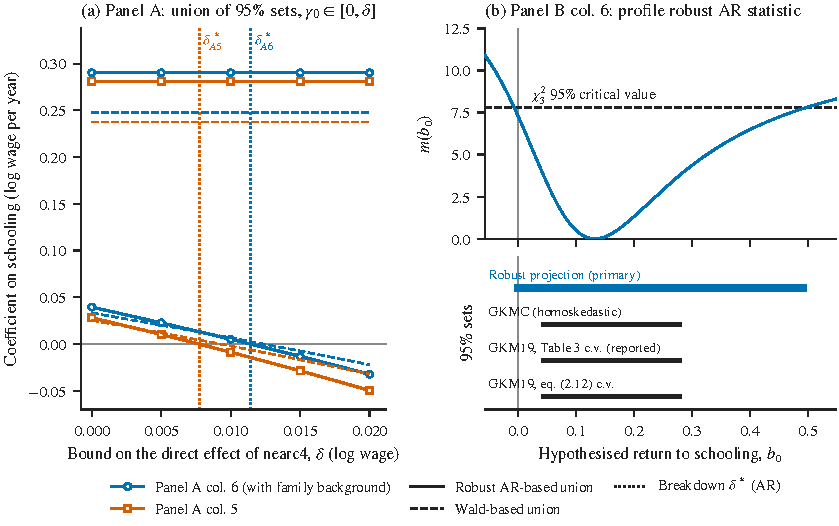
\includegraphics[width=0.9\linewidth]{figures/chr.pdf}
\caption{\small \textbf{(a) Sensitivity of the Panel~A coefficient on schooling to a direct
effect of college proximity; (b) weak-instrument-robust inference on the return to schooling
in Card's basic specification.} $\delta$ and $\delta^*$ are in log-wage units (0.01 is one log
point). All men in the analysis sample,
$N = \NSample$. All sets are 95\% sets.
\emph{(a) Panel A specifications, which treat experience as exogenous. The quantity is the
Panel A coefficient on schooling, not the return to schooling.} For each bound $\delta$ on
the direct effect of college proximity on log wages, the lines show the bounds of the
Conley--Hansen--Rossi union. The union is taken over the direct effect
$\gamma_0 \in [0, \delta]$ of the heteroskedasticity-robust (HC1) Anderson--Rubin sets,
shown as solid lines through the full $\delta$ grid, with markers at
$\delta = 0, 0.005, \ldots, 0.020$. The Wald-based union is shown as dashed lines; it is
secondary and not robust to a weak instrument. Panel A column 6, with family background, is
in blue with circles. Panel A column 5 is in orange with squares. At $\delta = 0$ the union
is the H3(a) robust AR set: $[\ASixArLo, \ASixArHi]$ for column 6, and
$[\AFiveArLo, \AFiveArHi]$ for column 5. Dotted vertical lines mark the breakdown points,
the smallest $\delta$ at which the robust union first includes 0:
$\delta^* = \ASixPacoefChrBreakdown$ for column 6, which is $\ASixPacoefChrShare$ of its
reduced-form coefficient; and $\delta^* = \AFivePacoefChrBreakdown$, or
$\AFivePacoefChrShare$, for column 5. The Wald-based unions break down at
$\ASixPacoefChrWaldBreakdown$ and $\AFivePacoefChrWaldBreakdown$.
\emph{(b) Card's basic specification, Panel B column 6, which treats schooling, experience
and its square as endogenous. The quantity is the return to schooling.} The curve is the
profile robust Anderson--Rubin statistic $m(b_0)$, the minimum over the two experience
coefficients of the HC1 full-vector AR statistic. The dashed line is the chi-square(3) 95\%
critical value, 7.815. The bars below show the 95\% sets on the evaluated point list. The
robust projection set is the primary set, in blue: $[\BSixArRobLo, \BSixArRobHi]$, one
piece. It is valid under heteroskedasticity whatever the strength of the instruments, but
it is conservative, so it is wider than an exact-size test's set. It contains 0, so this
set does not establish a positive return; it does not show that the return is zero. The
three homoskedastic subvector AR sets are shown alongside and do not decide H3(b): GKMC,
$[\BSixArGkmcLo, \BSixArGkmcHi]$; GKM19 with Table 3 critical values, the reported GKM19
set, $[\BSixArGkmOneNineLo, \BSixArGkmOneNineHi]$; and GKM19 with the eq.~(2.12) quantile
from ivmodels, $[\BSixArGkmOneNineqLo, \BSixArGkmOneNineqHi]$. Their critical values are
close to the chi-square(1) value because $\kappa_1$ is large everywhere on the point list
(minimum $\BSixKappaOneMin$). The plotted window of $b_0$ is the span of the sets and 0,
padded by 10\%. The statistic and the sets were evaluated on $[-1, 1]$ and beyond, up to
$|b_0| = 10^5$; on that evaluated point list no set has a piece outside the window
(pieces narrower than the outer-grid spacing outside $[-1,1]$ could be missed).}
\label{fig:chr}
\end{figure}

Figure~\ref{fig:chr}(a) lets proximity raise log wages directly by up to $\delta$. For the
Panel~A column~6 coefficient on schooling the robust union first includes zero at
$\delta^* = \ASixPacoefChrBreakdown$ in log wage (about one log point), \ASixPacoefChrShare{} of the replicated
reduced-form coefficient; for column~5 at \AFivePacoefChrBreakdown{}
(\AFivePacoefChrShare{}). With one instrument these are the lower 95\% limits of the robust
reduced forms, a little above the values about 0.010 and 0.007 predicted from Card's % crew:literal
published conventional numbers, because the HC1 standard errors of the reduced forms are
smaller than the conventional ones. Only the lower end of each union moves with $\delta$.
The Wald-based unions, not robust to a weak instrument, break down at
\ASixPacoefChrWaldBreakdown{} and \AFivePacoefChrWaldBreakdown{}.

No threshold was set; the reader must judge whether a direct effect of about one log point
is plausible. Two reference points exist, neither on the same model. In Card's Table~5,
which treats experience as endogenous, keeps family background and instruments schooling
with proximity interacted with parental education, the estimated direct effect of
proximity is 0.015 (0.029) or 0.013 (0.024) \citep{card1993nber}; both are above our % crew:literal
breakdown points and far from precise. With a control set that adds marital status,
\citet{steiner2025possibilistic} find that a positive return survives a direct effect of 1\%
but not of 2\% or 4\%. \citet{cinelli2025omitted} show for Panel~A column~5 that an omitted
variable explaining 0.67\% of the residual variation of both proximity and log earnings % crew:literal
suffices to make the IV estimate insignificant, and that confounding as strong as the SMSA
or Black indicator widens the AR interval to about [$-$0.02, 0.40]. Other work finds no significant % crew:literal
direct effect in its preferred specifications: principal-stratification reanalyses that
drop the exclusion restriction find none for always- or never-takers, with wide intervals
and a binary intermediate variable, although one of Luo et al.'s specifications that the
authors regard as misspecified gives a significantly negative never-taker effect
\citep{jiang2022multiply,luo2024identification}. Tests of the testable implications of
instrument validity with schooling binarised give mixed results: as reported by
\citet{carr2021testing}, the test of \citet{kitagawa2015test} rejects Card's instrument
without covariates, while Carr and Kitagawa do not reject when conditioning on Card's full
covariate set.

\subsection{IV versus OLS (H5)}
\label{sec:h5}

The Panel~A column~6 2SLS coefficient exceeds its OLS counterpart by \ASixPacoefDiff{}
(standard error \ASixPacoefDiffSe{}), with a 95\% Wald interval of [\ASixPacoefDiffLo,
\ASixPacoefDiffHi] that is not robust to a weak instrument; the robust control-function
$t$ is \ASixPacoefCfT{} ($p = \ASixPacoefCfP$), so equality is not rejected. For column~5 the
difference is \AFivePacoefDiff{} (\AFivePacoefDiffSe{}), interval [\AFivePacoefDiffLo,
\AFivePacoefDiffHi], $t = \AFivePacoefCfT$ ($p = \AFivePacoefCfP$). The conventional Hausman
$t$ statistics, \ASixPacoefHausmanTConv{} and \AFivePacoefHausmanTConv{}, agree with Card's
statement that the gap could be sampling error. Both OLS estimates lie inside the robust AR
sets for the corresponding Panel~A coefficients. The non-rejection is uninformative rather
than evidence of equality: the intervals are wide relative to the estimated differences,
and the minimum detectable difference fixed in advance was about 0.154. % crew:literal

\section{Robustness: the report-only checks}
\label{sec:robust}

% Report-only checks: r-age1419, r-balance, r-cluster. Published numbers on crew:literal lines.
\begin{table}[tbp]
\centering
\small
\caption{Report-only checks fixed in the design. None of them could change a
specification, a standard-error formula or a claim.}
\label{tab:checks}
\begin{tabular}{@{}llll@{}}
\toprule
\multicolumn{4}{@{}l}{\emph{(a) Men aged 14--19 in 1966, Card's basic specification (WP 4483 Table~4, row~7)}} \\
 & Published & Replicated & Match \\
N & 2,037 & \YoungN{} & yes \\ % crew:literal
2SLS, schooling (conventional SE) & 0.094 (0.064) & \YoungIv{} (\YoungIvSe{}) & yes, yes \\ % crew:literal
\quad 95\% Wald interval & -- & [\YoungIvLo, \YoungIvHi] & \\
OLS, schooling (conventional SE) & 0.076 (0.006) & \YoungOls{} (\YoungOlsSe{}) & no, yes \\ % crew:literal
\midrule
\multicolumn{4}{@{}l}{\emph{(b) Balance: coefficient on college proximity, HC1 standard errors}} \\
Outcome & Coefficient (SE) & In SD units & N \\
KWW score, men aged 14--15 in 1966 & \BalKwwYoung{} (\BalKwwYoungSe{}) & \BalKwwYoungSdu{} & \BalKwwYoungN{} \\
KWW score, all men (descriptive only) & \BalKwwAll{} (\BalKwwAllSe{}) & \BalKwwAllSdu{} & \NSample{} \\
School-record IQ, where recorded & \BalIq{} (\BalIqSe{}) & \BalIqSdu{} & \BalIqN{} \\
Share with IQ recorded, near minus not near & \IqObsDiff{} (\IqObsDiffSe{}) & & \NSample{} \\
\midrule
\multicolumn{4}{@{}l}{\emph{(c) CR1 standard errors clustered on region-1966 $\times$ SMSA-1966 cells (Panel A)}} \\
 & A(6) & A(5) & \\
First stage: clustered SE (ratio to HC1) & \ASixFsSeCl{} (\ASixFsClRatio{}) & \AFiveFsSeCl{} (\AFiveFsClRatio{}) & \\
First stage: clustered $t$ & \ASixFsTCl{} & \AFiveFsTCl{} & \\
Reduced form: clustered SE (ratio to HC1) & \ASixRfSeCl{} (\ASixRfClRatio{}) & \AFiveRfSeCl{} (\AFiveRfClRatio{}) & \\
Reduced form: clustered $t$ & \ASixRfTCl{} & \AFiveRfTCl{} & \\
\bottomrule
\end{tabular}

\smallskip
\begin{minipage}{0.95\linewidth}
\footnotesize
\emph{Notes.} (a) The interval is the estimate $\pm 1.959964$ times the conventional SE.
(b) Controls: for the 14--15-year-olds, the base controls without experience, family
background and an indicator for age 25 in 1976; otherwise age, age squared, the base
controls without experience and family background. KWW is the Knowledge of the World of
Work score from the 1966 interview. (c) \NClusters{} cells; the smallest has
\MinClusterSize{} men, and \NClustersUnderThirty{} has fewer than 30. Critical value
$t(0.975, G-1) = \TCritCl{}$. With so few, unequal cells, CR1 can itself over-reject.
\end{minipage}
\end{table}


\paragraph{Men aged 14--19 in 1966.} Older men may have moved near a college by 1966 for
college itself. Restricting Card's basic specification to men aged 14--19 in 1966
(Table~\ref{tab:checks}a) reproduces Card's N, \YoungN{}, and his IV estimate,
\YoungIv{} (\YoungIvSe{}). Its 95\% interval, [\YoungIvLo, \YoungIvHi], includes zero. For
the full sample we compare the estimate \IvReturn{} (\IvReturnSe{}) and its H3(b) set rather
than a Wald interval (deviation D6). The subsample OLS estimate, \YoungOls{}, does not
reproduce Card's 0.076; we did not diagnose this and ran nothing further. % crew:literal

\paragraph{Balance.} For men aged 14--15 in 1966, before any college, the coefficient of
proximity on the KWW score is \BalKwwYoung{} points (\BalKwwYoungSe{}), \BalKwwYoungSdu{}
standard deviations, on \BalKwwYoungN{} men; on school-record IQ it is \BalIq{}
(\BalIqSe{}), \BalIqSdu{} standard deviations, on \BalIqN{} men. Neither is distinguishable
from zero, so these checks do not show selection on measured ability. Two qualifications
weaken that reading. The 14--15-year-old sample is small, so the check has little power.
And IQ is recorded more often for men near a college, by \IqObsDiff{} (\IqObsDiffSe{}), so
the IQ subsample may be selected on proximity. The KWW coefficient for all men,
\BalKwwAll{} (\BalKwwAllSe{}), is descriptive only: a valid instrument would also raise it
through schooling completed by 1966.

\paragraph{Clustering.} Proximity is assigned by county, and the file has no county
identifier (deviation D1). Clustering on the \NClusters{} region-1966 $\times$ SMSA-1966
cells, the finest geography available, gives reduced-form standard errors smaller than HC1
(ratios \ASixRfClRatio{} and \AFiveRfClRatio{}) and clustered $t$ statistics of
\ASixRfTCl{} and \AFiveRfTCl{} against a critical value of \TCritCl{}. By the reading fixed in
advance this is not reported as robustness to county-level dependence: with so few,
unequal cells CR1 can itself over-reject. The first stage behaves differently in the two
columns. For column~5 the clustered first-stage standard error is \AFiveFsClRatio{} times
the HC1 one (clustered $t$ \AFiveFsTCl{}), so a clustered first-stage $F$ is below both H2
thresholds and below the HC1 effective $F$; for column~6 the ratio is \ASixFsClRatio{}
(clustered $t$ \ASixFsTCl{}), which puts a clustered $F$ between the two thresholds. Clustering
thus weakens the instrument-strength reading for column~5.

\section{Conclusion}
\label{sec:conclusion}

From Card's public file, the 2SLS and OLS estimates of his basic specification, every
Panel~A estimate and both OLS columns are reproduced at the printed precision. The \HOneMisses{}
misses are all in Panel~B's first-stage and reduced-form columns, and a post hoc diagnostic
suggests these columns keep experience in the equation, instrumented by age; the
diagnostic is consistent with Card's printed numbers but does not prove how they were
computed.

The inferential conclusions are narrower than the point estimates suggest. For Card's basic
specification, heteroskedasticity-robust inference that does not rely on instrument strength
does not establish a positive return to schooling; the test used is conservative, and the
homoskedastic subvector sets, which exclude zero, do not control size under
heteroskedasticity. For the Panel~A coefficient, which assumes experience exogenous, the
robust AR sets lie above zero, but the first stage is weak by conventional thresholds, the
sign survives only a direct effect of proximity of about one log point (the robust
reduced-form lower limit restated), and the 2SLS and OLS coefficients cannot be told apart.
None of these estimates is the average return to schooling for all men, and on these data
even the weighted-average reading needs conditions that are in doubt. The natural next step
is a heteroskedasticity-robust subvector test with correct asymptotic size and fewer
degrees of freedom than the projection, such as that of \citet{guggenberger2024powerful}, on Card's basic specification.

\section*{Limitations and deviations from the approved design}
\label{sec:deviations}

\paragraph{Limitations.}
\begin{itemize}
\item \emph{Independence across men.} Proximity varies by county, but no statistic can be
clustered by county (D1). Every standard error, AR set and breakdown point may be too
narrow; the cell-level clustering in Section~\ref{sec:robust} is only a one-directional
warning.
\item \emph{The Panel~A assumption.} H2, H3(a), H4 and H5 concern the Panel~A coefficient,
which treats experience as exogenous although experience contains schooling. Only H3(b)
concerns Card's basic specification (D2).
\item \emph{Conservative primary set.} The H3(b) decision rests on a projection set; a
robust subvector test with correct asymptotic size and fewer degrees of freedom was not
available to us in Python and was not implemented.
\item \emph{Untested exclusions.} The age exclusion in Panel~B is maintained, not tested.
The proximity exclusion is examined only through a breakdown point, balance checks with
little power or a selected sample, and the literature.
\item \emph{Interpretation.} The 2SLS coefficient's weighted-average reading needs
monotonicity and rich covariates, both in doubt on these data, and the complier results do
not directly apply when experience is also instrumented.
\item \emph{Sources.} The 1995 chapter was not read; the targets are WP 4483's printed
values. The working paper's tables were read from page images of a scan.
\item \emph{Unexplained misses.} The OLS estimate for men aged 14--19 is not reproduced
and not diagnosed, and the cause of the Black-share miss in Table~\ref{tab:sumstats} is
unknown.
\end{itemize}

\paragraph{Deviations.}
\begin{itemize}
\item \textbf{D1.} The track rule to cluster at the level of treatment cannot be followed:
\var{nls.dat} has no county or sampling-unit identifier. H1 uses Card's unclustered
standard errors; H2--H5 use HC1.
\item \textbf{D2.} Card's basic specification gets subvector AR sets (H3b) but no
instrument-strength test, exclusion breakdown or IV--OLS test; those are on Panel~A, which
the paper never calls Card's basic specification.
\item \textbf{D3} (recorded before any analysis run, after the first code review). Two
in-run agreement checks with \var{ivmodels} were implemented differently from the design's
wording: pointwise agreement fails the run only for $|b_0| \le 1$, because \var{ivmodels}
loses precision at large $|b_0|$; and the 20 check points use equally spaced $b_0$ values.
Neither changes an estimate, set or decision rule.
\item \textbf{D4} (post hoc, decided after the H1 runs and before the results review). The
report-only diagnostic of Panel~B columns 1--4 (Section~\ref{sec:diag}). It changes no H1
target, count or claim of the approved plan.
\item \textbf{D5} (fixed before the SAS-listing run). A failure rule for the listing check;
it was not needed.
\item \textbf{D6} (after the second results review). The plan asked for the age 14--19 and
full-sample estimates with two confidence intervals; the full sample is reported as
estimate and standard error with the H3(b) set as its interval, because no full-sample
interval was written as a run metric. No run was added.
\item \textbf{D7} (added at the paper stage, after the results gate). One descriptive
analysis run, \var{describe-sample}, recomputes the Table~1 items of the wage sample
(Table~\ref{tab:sumstats}) so that they can be reported as result claims; it changes no
estimate, decision or count. Its claims never passed a results review.
\item \textbf{D8} (paper stage, with the human author's consent in chat). The two axis
labels of the figure said ``log points'' for values in log-wage units. The labels alone
were corrected and the figure run repeated without a further code review, because the four
code-review rounds the protocol allows had been used; no statistic, check or input changed.
This is the one analysis run not covered by a passing code review.
\item \textbf{Timing.} The synthetic-data checks of the estimators, the figure code and the
first code review were planned before the design gate but took place after it, still before
any analysis run.
\end{itemize}

\section*{AI-use statement}

This paper was drafted by a crew of AI research-assistant agents
(Free-Research-Crew, protocol v0.2) under the direction of the human author, Bryce Wang.
He approved the research question (2026-11-20, 16:53 UTC), the design (2026-11-20,
17:49 UTC) and the results (2026-11-21, 02:17 UTC), each in chat after
reading the Reviewer's verdict. The manuscript itself is subject to the submission gate. He takes responsibility for the paper's content.

% Counts are macros from process.tex (`crew.py numbers`); who did what is taken from
% log.jsonl and reviews/.
\begin{itemize}
  \item \textbf{Roles and models.} Every role (PI, Scout, Designer, Data RA, Econometrician,
        Figures RA, Writer, Reviewer and Replicator) runs on Claude Opus 5.5
        (\texttt{claude-opus-5-5}) in Claude Code, each role as a separate agent. The PI
        drafted the question and hypotheses, recorded deviations D3--D8, and decided D7 and, with the human author's consent, D8; the Scout
        found and verified the sources and transcribed the published targets; the Designer
        wrote the design; the Data RA fetched and prepared the data and, at the paper stage, wrote and
        executed the descriptive run behind the summary-statistics table (D7); the Econometrician
        wrote and tested the estimation code, executed the analysis runs, including the
        post hoc diagnostic and the SAS-listing check, and wrote the result claims; the
        Figures RA drew the figure; the Writer drafted this paper from the claims; the
        Replicator ran the clean rerun. The PI's brief to each role is
        archived in \texttt{briefs/}.
  \item \textbf{Review.} The Reviewer ran \CrewReviewRounds{} rounds on
        \CrewReviewerModels{} (\CrewReviewIndependence{}: a new context in every round, the
        same model family as the other roles): \CrewRoundsQuestion{} on the question,
        \CrewRoundsLiterature{} on the literature, \CrewRoundsDesign{} on the design,
        \CrewRoundsCode{} on the code, \CrewRoundsResults{} on the results and
        \CrewRoundsPaper{} on the paper. It raised \CrewFindingsCritical{} critical,
        \CrewFindingsMajor{} major and \CrewFindingsMinor{} minor distinct findings (a
        finding carried into a later round is counted once, at its latest severity). The last round of each completed stage passed, with minor findings answered
        before the next gate. A code review passed before every analysis run except the D8 figure rerun, including
        separate rounds for the post hoc diagnostic, the SAS-listing check and the D7
        descriptive run.
  \item \textbf{Runs.} \CrewRuns{} runs in the ledger (\CrewRunsAnalysis{} analysis,
        \CrewRunsDataPrep{} data preparation); \CrewRunsSuperseded{} were replaced by a
        later run with the same id and archived (data-preparation and figure runs only; no run
        behind a result claim was replaced); \CrewRunsUnreviewed{} analysis
        run was not covered by a passing code review: the figure run repeated at the paper
        stage to correct its axis-label units only (deviation D8), with the human author's
        consent in chat, after the four code-review rounds had been used.
  \item \textbf{Replication.} The Replicator's clean rerun (\texttt{crew.py rerun}, in a
        fresh environment built from \texttt{code/requirements.txt}) has status
        \CrewRerunStatus{}: \CrewRerunReproduced{} of \CrewRerunTotal{} runs reproduced.
        Whether the work can be rerun from scratch is what this record states, not
        something the authoring roles assert.
  \item \textbf{Findings accepted over the Reviewer's objection.} None.
  \item \textbf{Evidence.} Every result number in the text, the tables and the figure caption
        is a macro generated from the metrics of a logged run. The numbers typed by hand are
        design facts fixed before any analysis run (critical values, targets, the
        pre-registered minimum detectable difference), published numbers quoted next to
        their replication, numbers from the literature quoted as the Scout's source notes
        record them (for example first-stage $F$ statistics, intervals and direct-effect
        estimates of earlier studies), and process facts such as dates. Card's SAS listing,
        which holds regression output, was left unopened until every claim of the approved
        plan was written. Claims added later came from metrics already written by earlier
        runs (results review), from the D7 descriptive run, or, at the paper review, from
        metrics already written (target and item counts, including the listing run's own,
        the KWW sample size, and the post hoc, descriptive homoskedastic statistic at zero);
        some claim texts were reworded at the paper stage. No claim value changed after the
        listing was read. Every
        citation was checked against its source by the Scout; the verification method for
        each entry (full text, abstract or DOI resolution) is recorded in
        \texttt{sources/sources.json}, and the paper cites each source for no more than was
        read. The full workspace, with the plan, run ledger and notes, code, data manifest,
        reviews, briefs and source notes, is at
        \url{https://github.com/brycewang-stanford/Free-Research-Crew/tree/main/gallery/ss-card-proximity}.
\end{itemize}


\bibliographystyle{plainnat-keepcase}
\bibliography{../refs}

\end{document}
